\documentclass[10pt]{article}

\usepackage{multicol}
\usepackage{graphicx,amsmath,listings,hyperref,color,appendix,geometry}
\usepackage[english]{babel}
\usepackage{graphicx}
\usepackage{float}
\usepackage{mathtools}
\usepackage{fullpage}
\usepackage{listings,color}
\usepackage{xcolor}


%%\renewcommand{\bibsection}{}

\newfloat{listing}{H}{lop}
\floatname{listing}{Listing}

\renewcommand\lstlistingname{Appendices} % Change language of section name

\begin{document} 
\begin{figure}[!bh]
 	\begin{center}
 	 
 		\huge \title{Impacts of the HTTP/2 protocol for large scale web environments}
		\author{Martin Leucht, James Gratchoff \\
		Master SNE \\ University of Amsterdam} 
		
\includegraphics{images/uva.jpeg}
	\maketitle 
		\label{sec:uva}
	\end{center}
\end{figure}
\pagenumbering{gobble}
\setlength{\columnsep}{2cm}
\def\columnseprulecolor{\color{blue}}
 
\newpage
\begin{abstract}
This paper compares version 1.1 and version 2 of the HTTP protocol. Both versions have been tested with TLS enabled. The main purpose is to show differences in terms of latency, header size, bandwidth utilisation and server performance between both protocol versions. In order to measure and compare the characteristics of the protocols, a benchmark setup has been developed. On server side different webserver implementaions were deployed in order to serve both protocol versions. HTTP clients are located around the world to represent different RTTs. The tool used for the protocol benchmarking is h2load. A script that calls h2load and is capable to provide our measurement requirements was developed. The results identify a clear improvement of the HTTP/2 protocol in terms of latency times and decreasing header sizes. Moreover the server performance will benefit from improvements that have been introduced in HTTP/2.
\end{abstract}

\newpage
\tableofcontents

\pagenumbering{arabic}
\newpage
%%\section*{Abstract}
\label{chap:intro}
\textit{This paper compares the version 1.1 and 2 of the HTTP protocol. The two version have been tested with TLS enabled. The purpose is to show the difference in terms of latency, header size, bandwidth utilisation and server performance. To do that a benchmark have been performed on a native HTTP2 server (nghttp) that is able to manage HTTP/1.1 request (on apache2) thanks to a proxy (nghttpx). Clients are located around the world to represent different RTTs. The tool used for the benchmark is h2load. The results shows a clear improvement in latency and header size with HTTP/2. Moreover the server performs better and uses less resources with HTTP/2.}
\newpage
\section{Introduction}
\label{chap:intro}
Specified by the IETF in 1999 in multiple RFCs(7230-7235\cite{RFC723x}), HTTP/1.1 is a standard protocol for web-browsing. HTTP is the essence of the web and most of the users are using this protocol on a daily basis. After more than 15 years of use it was time for a change. All the workarounds not to slow the HTTP/1.1 protocol have to be forgotten as on February the 18th 2015, the specification \cite{http2} for the new HTTP protocol HTTP/2 (and HPACK\cite{hpack}), has been formally approved by the IESG and is on the way to become an RFC standard.   \\
The main focus during the development period of the successor of HTTP/1.1 was to improve the performance, and thus provide a better user experience. The performance improvement is based on how the packets are sent over the wire within a HTTP/2 session. HTTP/2 data is sent in binary format and instead of creating a single TCP session per element retrieved, HTTP/2 use TCP streams that are multiplexed and can be prioritized. The purpose of this technique is to reduce to one the number of TCP sessions created every time a user access a web page. Concerning security, HTTP/2 will not make the use of TLS mandatory. However, leading browsers firms, such as Mozilla Firefox and Google Chrome have already mentioned that HTTP/2 will only be implemented over TLS. Thus ensuring that the data will be encrypted between two end parties. HTTP/2 introduces several other new features that will be presented in this paper. \\
There are already web client and server implementations\cite{http2-imp} that support the final HTTP/2 specification. This research is intending to show what are the impacts of implementing HTTP/2 with TLS compared to HTTPS in a large environment. A benchmark will be performed on a physical web server that will be tested with a high number of virtual clients located at different places around the world to outline the impact of the round trip time (RTT) on both version of the protocol and to see which performs the best. The research will draw conclusions on what impacts does the new protocol can have on large web service providers infrastructure.
\section{Research Questions}
\label{chap:rq}

How do the new features of the  HTTP/2 protocol improve the performance for frequently visited webpages/webserver?

That question can be narrowed down to some sub questions.
\begin{itemize}
\item What are possible drawbacks that can occur for large web service providers when switching from HTTP/1.1 to HTTP/2 ?
\item What is the predictable impact that could be related to changes in the infrastructure of Web service providers?
\item What is the difference in bandwidth utilization between HTTP/1.1 and HTTP/2 considering the size ratio of header and data for multiple concurrent sessions on a server?
\item How much can HTTP/2 decrease the amount of data when considering header compression and using multiple streams within one TCP Session compared to HTTP/1.1 on a server ?
\item What is the impact regarding the response time experienced by a client when the number of concurrent requests / clients increases seen from three different geographical locations?
\item What is the impact to the load and CPU utilization to the server when conducting the benchmark tests?
\end{itemize}
\section{Related work}
\label{relwork}
The brand new IETF accepted HTTP2 protocol has been based on the SPDY protocol developed mainly by Google. As shown by Google \cite{google2x}, the SPDY protocol is answering its expectation by reducing the loading time of web pages by 55\%. Other people have tried to look into the protocol and one of the most interesting is Herve Servy's post\cite{servy}. Servy evaluated the performance of the web servers implementing the SPDY protocol comparing it to HTTP1.1 and HTTPS. The load testing tool used for this benchmark was the NeoLoad 4.1.2. His results showed that the implementation of SPDY increases by a factor of 6 the number concurrent of users possible before errors start showing up in comparison to HTTP and HTTPS. The fact that SPDY is using a single connection for all requests induce that the clients are using one worker instead of multiple in HTTP and HTTPS. That makes the server able to handle more users with the same amount of worker. Servy also looked into the repercussion of the SPDY implementation in terms of CPU and memory consumption at the server side. Compared to HTTP, SPDY requests consume less memory but more CPU. However compared to HTTPS SPDY requests consume less memory and CPU usage.
A contradictory study showing some boundaries of implementing SPDY has been done by Podjarny\cite{podiatry}, he shows that most of the website uses different domains and as SPDY works on a per-domain basis it does not necessarily help it to be faster. Finally, Wang et al.\cite{wang} have investigated the performance of SPDY for the improvements of the protocol compared to HTTP. This study highlight that SPDY is much faster as benefiting from the single TCP connection mechanism. However they also mention that SPDY degrades under high packet loss compared to HTTP. 
Concerning the new standard HTTP2 a few benchmark have been done by the creator of the different client/server platforms. They all fall down in the same conclusion for SPDY. However no study shows its impact on the infrastructure.
\section{Scope}
\label{scope}
\section{Approach and Methods}
\label{sec:approach_and_methods}



\subsection{Measurement}
\subsubsection{Measurement Parameter}
\label{subsec:measurements}
To perform various measurements that reflect realistic scenarios a large web content provider will encounter, a topology consisting of several components was composed. As HTTP client machines, Amazon AWS microinstance VMs \cite{amazon} located at different geographical locations (Europe, North America and Asia) are used. Different geographical locations used on client side, ensure to perform measurements seen from different magnitudes of Round Trip Times towards the destination web server located in Amsterdam. On server side two TLS enabled webserver instances are running on one physical machnine in order to conduct measurements for both protocols - HTTP/1.1 and HTTP/2. Three reference HTML pages of different sizes and different numbers of statically linked resources have been created to be compared. These pages reflect the sizes that can be encountered in most common websites and has been derived from top 100 websites statistics \cite{httparchive}. The appropriate web page sizes including the number of resources are listed in Table \ref{table:pages}.

\begin{table}[h]
	\centering
\begin{tabular}{ | c | c | c | }

\hline
\textbf{Web Page} & \textbf{Size (kB)} & \textbf{Number of links}\\ \hline \hline
small.html &  20 & 2 \\ \hline
medium.html &  600 & 7\\ \hline 
large.html &  1600 & 54 \\
\hline
\end{tabular}
\caption{different Web Pages}
\label{table:pages}
\end{table}

So far, we have defined different static parameters that will be applied while performing the measurement. These parameters include different Round Trip Times (RTTs) and different webpage sizes.  
To simulate varying and realistic load scenarios on the server, the number of clients and thereby the number of requests towards the webservers is incremented during each test starting from one client upto maximal 750 clients in parallel.
\\  
\subsubsection{Measurement Tools}
It is essential to choose and implement the right tool and method to measure the response/request times characteristics of the HTTP/1.1 and HTTP/2 protocol and to be able to compare them with each other. Thus, the bechmarking tool was chosen carefully and with respect to retrieve accurate measurement data that can be used to compare both HTTP versions with each other. 
H2load \cite{h2load} was elected as the best candidate for that purpose. It has been developed to run benchmarking tests against HTTP/2 enabled webservers. 
It can also be used to conduct measurements against HTTP/1.1 enabled web servers if, like in that case, a HTTP/2 - HTTP/1.1 reverse proxy is used that is capable to translate HTTP/2 requests into HTTP/1.1 requests on server side. 
It is possible to start h2load with a file option, that includes a list of URIs that each measurement will request in parallel. H2load returns after each measurement round accurate and valuable data, like the retrieved  amount of header and body data in bytes per request. Furthermore it returns the minimum, maximum and mean round trip time for each web page request and the actual performance in requests/second. 
\\
\subsubsection{Measurement Methods}
In order to collect statistical analysable data, all measurements are performed with twenty repetitions. A wrapper script was created that performs the measurements using h2load, does mean calculations on the data and writes them into a file. The data is later processed for visualizing round trip times and other measurements. The wrapper script can be found at the end of that report as part of the appendices. 
\\
It is important to notice that the main difference between HTTP/1.1 and HTTP/2 sessions is based on the number of created TCP sessions on server side. A HTTP/1.1 client (e.g. web browser) opens for each HTML link that is present in a HTML webpage a separate TCP session to the webserver. In contrast to HTTP/1.1, the new HTTP/2 protocol opens one single TCP session towards the server and multiplexes all requested data over multiple streams within a single TCP session. Thus, the maximum number of concurrent streams for each HTTP/2 session is set equal to the amount of requested URIs in all measurements. Figure \ref{fig:httpwatch} shows HTTP/1.1 GET requests in order to get the entire set of resources the reference webpage (large.html) includes.


\begin{figure}[H]
	\centering
	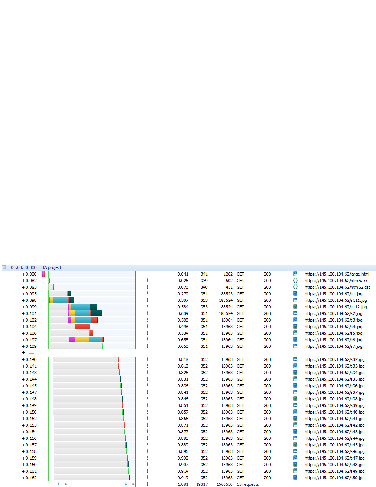
\includegraphics[scale=2,trim=0.0cm .0cm .0cm 4.5cm,clip]{images/http.pdf}
	\caption{HTTP/1.1 GET requests for large.html}
	\label{fig:httpwatch}
\end{figure}

HTTP/2 handles all GET requests in a single TCP connection by using multiple streams \textit{s}, thus the expected number of TCP connections \textit{t} will be equal to the number of concurrent simulated clients \textit{n}. For HTTP/1.1  we expect the number of TCP connection \textit{t} as a function of the product of concurrent clients \textit{n} by the requested number of HTML links \textit{l}. Thus we can describe the number of TCP sessions for HTTP/1.1 as \begin{equation}
t=f(n)=n*l \qquad \text{and} \qquad l \geq 1\end{equation} and for HTTP/2 as \begin{equation} t=f(n)=n \qquad \text{and} \qquad s=l; l\geq 1; s \in n \end{equation}

That results in Table \ref{table:tcpconnects} which shows the expected numbers of TCP connections towards the webserver during some stages in the measurements with an assumed number of \textit{l=55} HTML links per page request.

\begin{table}[h]
	\centering
\begin{tabular}{ | c | c | c | }

\hline
\textbf{clients/requests \textit{n}} &\textbf{\textit{t} (HTTP/2)} &\textbf{\textit{t} (HTTP/1.1)}\\ \hline \hline
1 & 1 & 55 \\ \hline
10 & 10 & 550\\ \hline
50 & 50 & 2750\\ \hline
150 & 150 & 8250\\ \hline
300 & 300 & 16500 \\ \hline
500 & 500 & 27500\\ \hline 
750 & 750 & 41250\\
\hline
\end{tabular}
\caption{Number of TCP connections HTTP/1.1 and HTTP/2}
\label{table:tcpconnects}
\end{table} 
%%\subsection{Overview}
\label{subsec:topology}
For our measurements we have setup a benchmark topology consisting of Amazon AWS microinstance \cite{amazon} clients located at different geographical locations (Europe, North America and Asia). That ensures to perform measurements seen from clients with  different Round Trip Times to the destination server located in Amsterdam. On the server side, in Amsterdam, different webserver implementations are used in order to conduct measurements for both protocols - HTTP/1.1 and HTTP/2. 
\\
Three reference HTML pages of different sizes and different numbers of statically linked resources have been created to be compared. These pages reflect the sizes that can be encountered in most common websites and has been derived from top 100 websites statistics \cite{httparchive}. The page sizes including all resources, are listed in Table \ref{table:pages}.

\begin{table}[h]
	\centering
\begin{tabular}{ | c | c | c | }

\hline
Web Page & Size (kB) & Number of statically linked resources\\ \hline \hline
small.html &  20 & 2 \\ \hline
medium.html &  600 & 7\\ \hline 
large.html &  1600 & 54 \\
\hline
\end{tabular}
\caption{different Web Pages}
\label{table:pages}
\end{table}

So far, we have defined different static parameters that will be applied while performing the measurement. These parameters include different Round Trip Times (RTTs) and different webpage sizes. To simulate varying and realistic load scenarios on the server, the number of clients and thereby the number of requests towards our webservers is incremented during each test from one client upto maximal 750 clients in parallel. Figure \ref{fig:httpwatch} shows all required HTTP/1.1 GET transactions in order to fetch the entire set of resources included in the large variant of the reference webpage (large.html).

\begin{figure}[H]
	\centering
	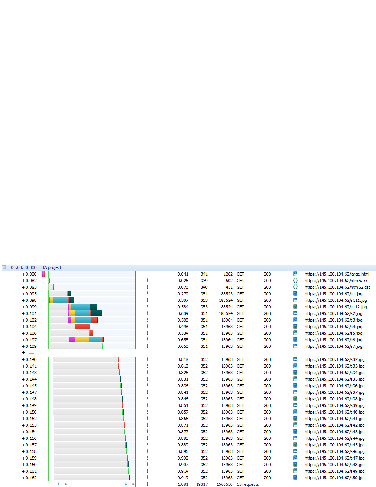
\includegraphics[scale=2]{images/http.pdf}
	\caption{Page Requests for large.html}
	\label{fig:httpwatch}
\end{figure}
  

It is essential to choose and implement the right tool to measure the response/request characteristics of the HTTP/1.1 and HTTP/2 protocol and to be able to compare them with each other. Thus, the bechmarking tool was chosen carefully and with respect to retrieve measurement data that can be used to compare both HTTP versions with each other. 
\\
H2load \cite{h2load} was the best candidate for that purpose. It has been developed to run test against HTTP/2 enabled webservers. i
It can also be used to conduct measurements against HTTP/1.1 enabled servers if, like in that case, a HTTP/2 - HTTP/1.1 reverse proxy is used taht is capable to translate HTTP/2 requests into HTTP/1.1 requests.    

\subsection{HTTP Server and Clients}
\label{subsec:server_client}
HTTP clients that conduct measurements from long distances are deployed using Amazon t2.micro instances. T2 instances provide a baseline level of CPU performance that is comparable to 2 vCPUs with the ability to burst above the baseline level \cite{amazon-ts}. For local tests within the OS3 network, XEN VM are used. Each virtual machine got 2 vCPUs and 2 Gigabyte RAM assigned. The clients are located in different geographical areas, resulting in different RTT times between clients and server. On each client h2load was compiled and the wrapper script uploaded. Table \ref{table:locations} shows all clients and their corresponding average round trip times to the server.

\begin{table}[h]
	\centering
\begin{tabular}{ | c | c | }

\hline
\textbf{Location} & \textbf{RTT in ms}\\ \hline \hline
Tokyo/Asia &  280\\ \hline
North Carolina/North America &  150\\ \hline 
Frankfurt am Main/Europe &  7\\ \hline
Amsterdam/Europe (local) &  0.3\\

\hline
\end{tabular}
\caption{RTT (in ms) per location}
\label{table:locations}
\end{table}

The server that provides access for the HTTP clients is not virtualized. It has 8 Intel Xeon CPUs (1,87GHz) and 8GB RAM installed. The web server has a public IPv4 address and is connected to the public internet via a 1 Gbit Ethernet interface. As HTTP/2 server nghttpd \cite{nghttp} version 0.76-DEV is used which listens on TCP port 8881. For HTTP/1.1 requests Apache2 \cite{apache2} in combination with nghttpx \cite{nghttpx} is used. The Apache2 configuration has been adjusted in order to allow the webserver to start a maximum number of 750 server worker processes. This adjustment was required because Apache starts multiple worker processes depending on the amount of request. and we discovered that the default configuration was not sufficient for our setup. Nghttpx is a reverse proxy and accepts HTTP/2, SPDY and HTTP/1.1 over SSL/TLS on TCP port 8443 via its front-end. The most recent version of nghttpx (0.76-DEV) at the moment that research was done is used. The protocol to the back-end is HTTP/1.1. The usage of an reverse proxy enables us to use our measurement tools without modification, although native HTTP/1.1 requests instead of using a reverse proxy would probably result in more accurate measurements. Since our time was very limited, we decided us to go for the reverse proxy option.


\newpage
\section{Results analysis}
\label{sec:results}
In that section the measurement results are presented and analysed. First the HTTP header sizes for HTTP/2 and HTTP/1.1 are compared against each other. Second, the results of the RTT measurements and the actual performed rate of requests per second with a growing number of concurrent clients are presented and discussed for each measurement separately. Finally an overview of the server utilization during the measurements is given for network bandwidth, CPU utilization and TCP sockets.  
\subsection{HTTP header size}
\label{subsec:header_size}

HTTP/2 uses HPACK \cite{hpack} as a header compression mechanism in order to decrease the amount of data for repetitive HTTP header information. Figure \ref{fig:headersize} shows the difference between HTTP/2 and HTTP/1.1 regarding the amount of header depending on the amount of clients.

\begin{figure}[H]
	\centering
	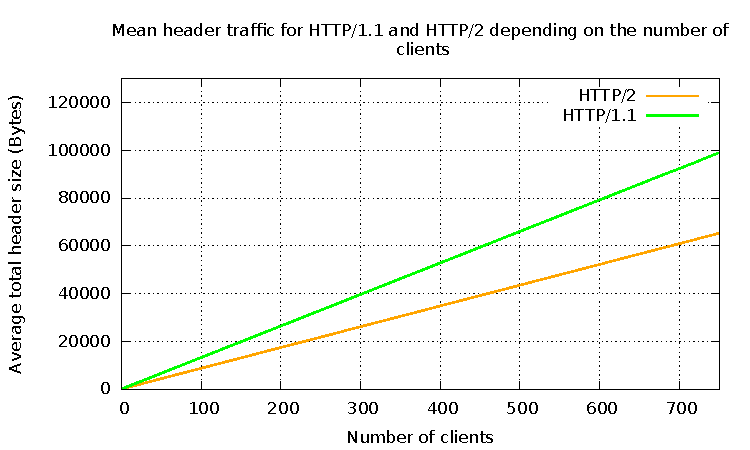
\includegraphics[scale=1,trim=0.0cm .0cm .0cm .0cm,clip]{images/headertraffic.pdf}
	\caption{header traffic in bytes for HTTP1.1 and HTTP/2}
	\label{fig:headersize}
\end{figure}

The result is a linear graph for both versions with a higher rate of growth for HTTP/1.1. It turns out that in our measurement set-up the amount of traffic produced to transmit HTTP headers is approximately 30\% lower for HTTP/2 compared to HTTP/1.1. 

\subsection{HTTP Round Trip Times and Request Rates}
\label{subsec:rtt}

In that section the RTT time seen from different locations with a growing number of clients is presented. Furthermore the performance in requests per second is shown. The test are shown by location ordered by decreasing distance to the server

\subsubsection{Tokyo/Asia}

The measurements in asia are performed with the highest RTT of 280 ms. The graph in Figure \ref{fig:latency-asia}  represents the data for 4 measurements by using for each HTTP version two different pages (20kB, 1600kB). The number of clients is incremented by one  from 1 to 750, while performing the measurements.

\begin{figure}[H]
	\centering
	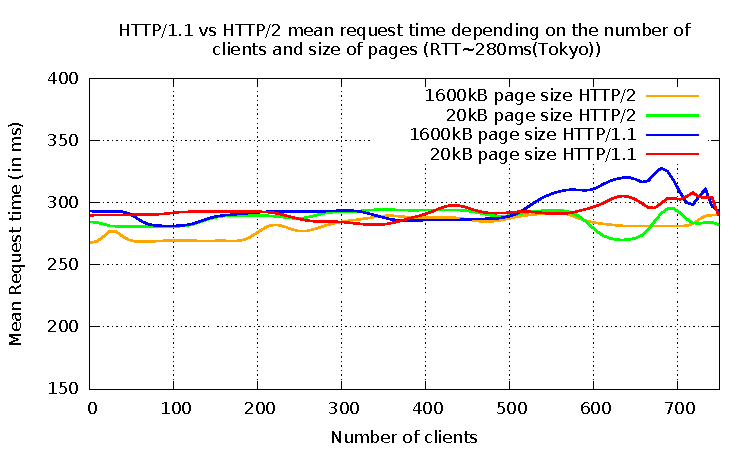
\includegraphics[scale=1,trim=0.0cm .0cm .0cm .0cm,clip]{images/latency-asia.pdf}
	\caption{Mean RTT measurements for Tokyo/Asia}
	\label{fig:latency-asia}
\end{figure}

A significant difference between both HTTP versions cannot be identified, although HTTP/2 is a few milliseconds faster during the measurements. The graph shows nearly a constant response time regardless if the number of clients increases. That can be explained by considering the rate of requests per seconds seen from the client in Tokyo. As more clients are added as more requests are beeing executed in approximately the same time. The graph in Figure \ref{fig:reqps-asia} shows that dependency.

\begin{figure}[H]
	\centering
	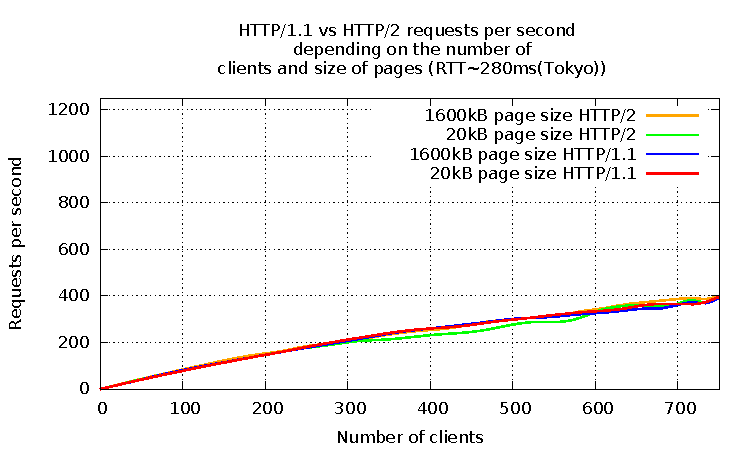
\includegraphics[scale=1,trim=0.0cm .0cm .0cm .0cm,clip]{images/reqps-asia.pdf}
	\caption{Mean Requests per second for Tokyo/Asia}
	\label{fig:reqps-asia}
\end{figure}

\subsubsection{Northcarolina/US}

The next measurements were taken from a client in North America/North Carolina with a measured base average RTT of 150ms and is shown in Figure \ref{fig:latency-na}. 

\begin{figure}[H]
	\centering
	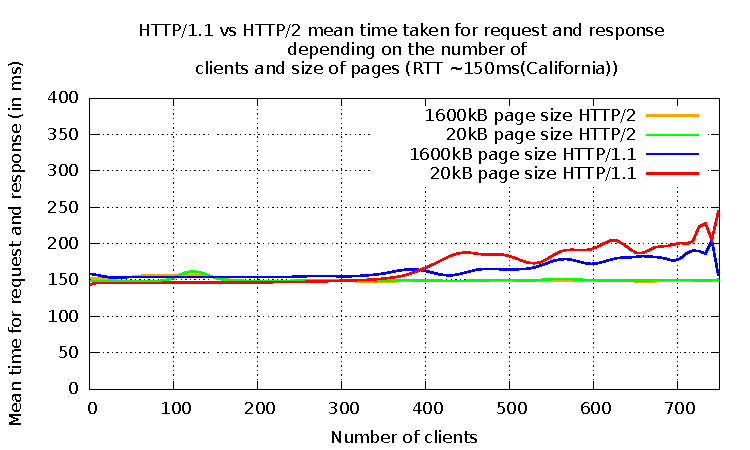
\includegraphics[scale=1,trim=0.0cm .0cm .0cm .0cm,clip]{images/latency-na.pdf}
	\caption{Mean RTT measurements for North Carolina/US}
	\label{fig:latency-na}
\end{figure}

The graph shows for HTTP/2 measurements, that the HTTP RTT is nearly almost equal to the measured base RTT. That means there is almost no jitter measurable and the RTT is constant for HTTP/2 requests regardless if the number of clients is raised or not. Moreover we see a growing HTTP/1.1 RTT starting from approximately 400 concurrent clients upwards. Figure \ref{fig:reqps-na} shows the corresponding request per second rate graph.

\begin{figure}[H]
	\centering
	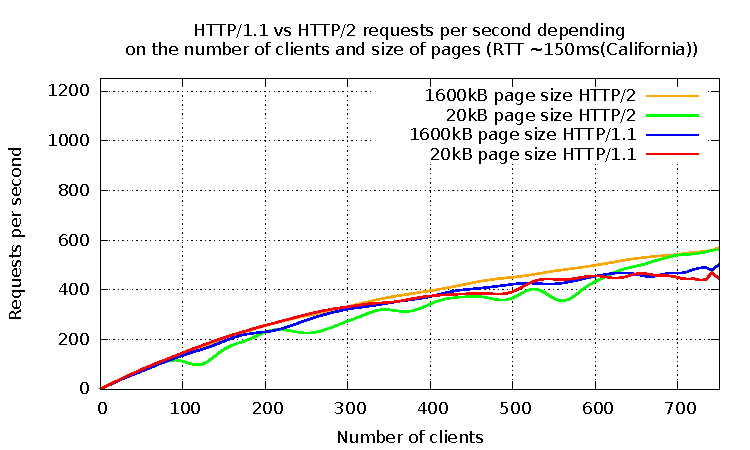
\includegraphics[scale=1,trim=0.0cm .0cm .0cm .0cm,clip]{images/reqps-na.pdf}
	\caption{Mean Requests per second for North Carolina/US}
	\label{fig:reqps-na}
\end{figure}

A slightly better request performance rate for HTTP/2 is the result of that mesurement. 

\subsubsection{Frankfurt am Main/Europe}

Measurements taken from a client in Frankfurt am Main/Germany represent a low latency link with approximately 7ms of base RTT. The graph for the HTTP RTTs is shown in Figure \ref{fig:latency-europe}.

\begin{figure}[H]
	\centering
	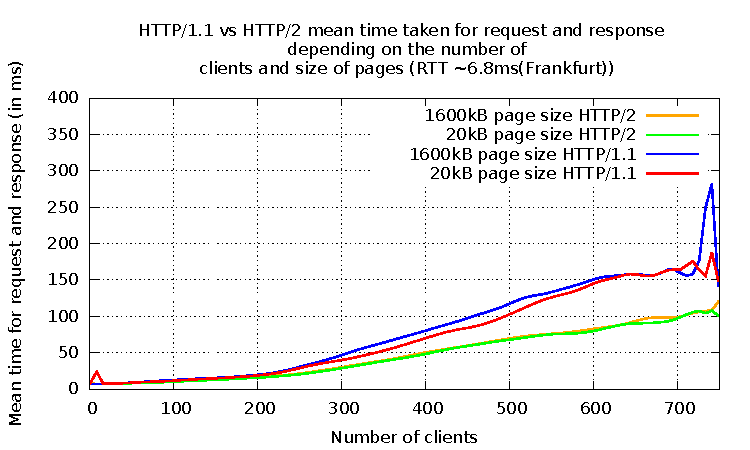
\includegraphics[scale=1,trim=0.0cm .0cm .0cm .0cm,clip]{images/latency-frankfurt.pdf}
	\caption{Mean RTT measurements for Frankfurt am Main/Europe}
	\label{fig:latency-europe}
\end{figure}

Compared to the previous measurements, the RTT graph looks different. Depending on the number of clients the RTT times grow nearly proportional. It is also a clear difference between HTTP/1.1 and HTTP/2 visible. The performed HTTP/2 mesurements show significanltly less growing upto approximately 100ms for 750 clients, whereas the HTTP/1.1 RTT is for all meaurements around 30\% slower ending up in a maximum of around 150ms. The  request rate graph shown in Figure \ref{fig:reqps-frankfurt} shows a different characteristic compared to the previous measurements.

\begin{figure}[H]
	\centering
	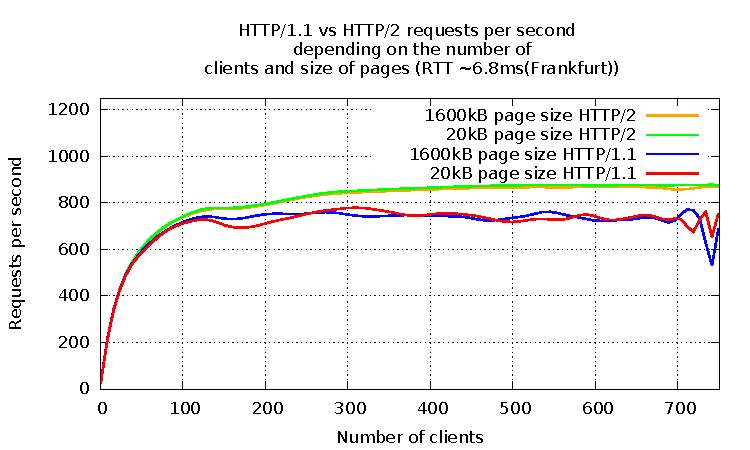
\includegraphics[scale=1,trim=0.0cm .0cm .0cm .0cm,clip]{images/reqps-frankfurt.pdf}
	\caption{Mean Requests per second for Frankfurt/Germany}
	\label{fig:reqps-frankfurt}
\end{figure}

It turns out that the request rate is identical to a asymptotic curve for all measurements. The server simply cannot handle more connection than approximately 800. That is also the reason that after 100 concurrent concurrent clients the request rate remains nearly static. It is again visible that HTTP/2 performs better compared to HTTP/1.1. The fact that the base RTT for that measurement is significantly less than in the previous measurement, leads to much more connections at the same time at the server and different performance graphs.

\subsubsection{Local/Amsterdam}

Finally we performed measurements within the OS3 network (RTT 0.3 ms). We conducted those tests in two different ways. First we did separate measurements for each protocol version and then we conducted parallel tests in order to simulate workloads on the server for HTTP/1.1 and HTTP/2 requests simultanaeous. Figure \ref{fig:latency-local} and Figure \ref{fig:reqps-local} show the graphs for the separate measurements.

\begin{figure}[H]
	\centering
	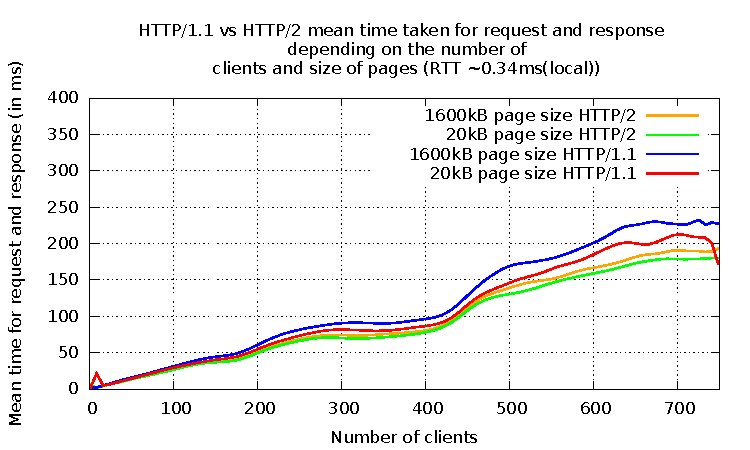
\includegraphics[scale=1,trim=0.0cm .0cm .0cm .0cm,clip]{images/latency-local.pdf}
	\caption{Mean RTT measurements for local/OS3 network}
	\label{fig:latency-local}
\end{figure}

\begin{figure}[H]
	\centering
	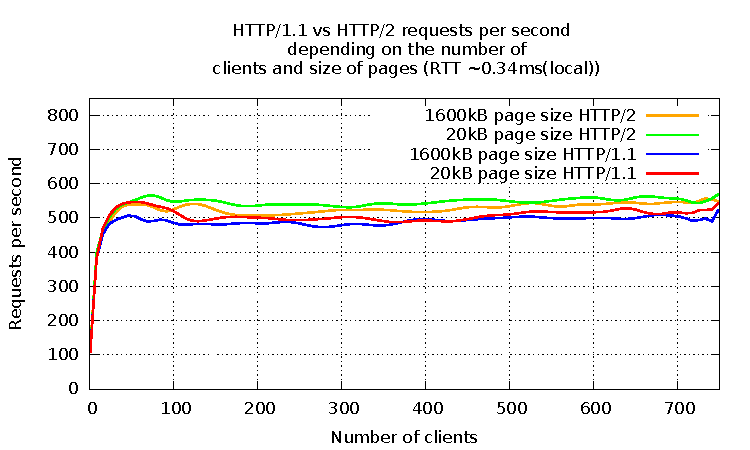
\includegraphics[scale=1,trim=0.0cm .0cm .0cm .0cm,clip]{images/reqps-local.pdf}
	\caption{Mean Requests per second for local/OS3 network}
	\label{fig:reqps-local}
\end{figure}

The graph characteristics is similar to the low latency link in Frankfurt. The difference between both measurements is the number of client needed to reach the server limit in terms or requests per second. The local measurement already reaches that limit at approximately 40 clients. That can be explained by the lower latency within the OS3 network.
\\
\\
As a last measurement we conducted parallel tests for HTTP/1.1 and HTTP/2. The related graphs are shown in Figure \ref{fig:latency-localv1vsv2} and Figure \ref{fig:reqps-localv1vsv2}

\begin{figure}[H]
	\centering
	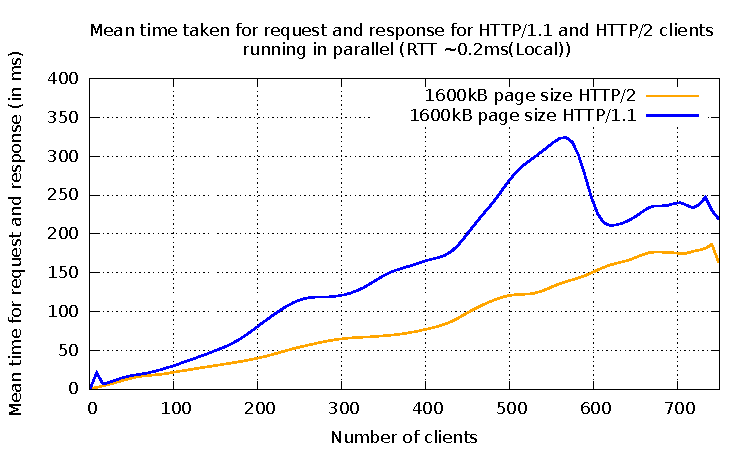
\includegraphics[scale=1,trim=0.0cm .0cm .0cm .0cm,clip]{images/latency-localv1vsv2.pdf}
	\caption{Mean RTT measurements for local parallel/OS3 network}
	\label{fig:latency-localv1vsv2}
\end{figure}

\begin{figure}[H]
	\centering
	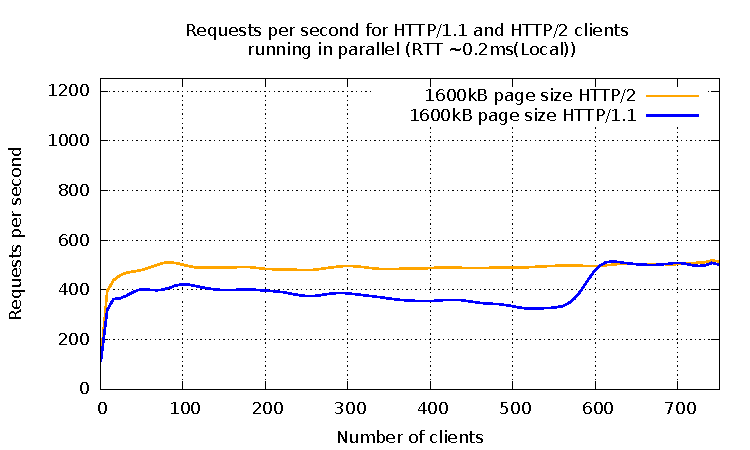
\includegraphics[scale=1,trim=0.0cm .0cm .0cm .0cm,clip]{images/reqps-localv1vsv2.pdf}
	\caption{Mean Requests per second for local parallel/OS3 network}
	\label{fig:reqps-localv1vsv2}
\end{figure}
 
The final result of the local parallel measurements shows again a significant difference between HTTP RTT times of both versions. HTTP/2 is clearly faster than HTTP/1.1. Figure \ref{fig:latency-localv1vsv2} shows a peak RTT for HTTP/1.1 at around 550 clients. At that moment the last HTTP/2 measurement was finished and afterwards the server was only busy with responding to HTTP/1.1 request. That is the reason for the decreasing RTT for HTTP/1.1 and the increasing number of requests per second starting  from that point.

\subsubsection{Mesurement analysis}

We can conclude that for almost all measurements the RTT time for HTTP/2 is significantly faster than for HTTP/1.1. That result is independent of the requested page size and also from the distance between client and server. For high latency links we discovered different characteristics regarding the request rate compared to low latency links (Frankfurt/Local). On low latency links (ca. 10ms) the number of requests per seconds grows much faster, which results in a quick saturation of the server to its maximum number of parallel requests. For high latency links a constant increase of RTT and request rate was measured for an increasing number of clients. In Figure \ref{fig:latency-all} all measured differences between HTTP/1.1 and HTTP/2 for all locations is shown. Lines above zero (y-axis) show a faster RTT for HTTP/2.

\begin{figure}[H]
	\centering
	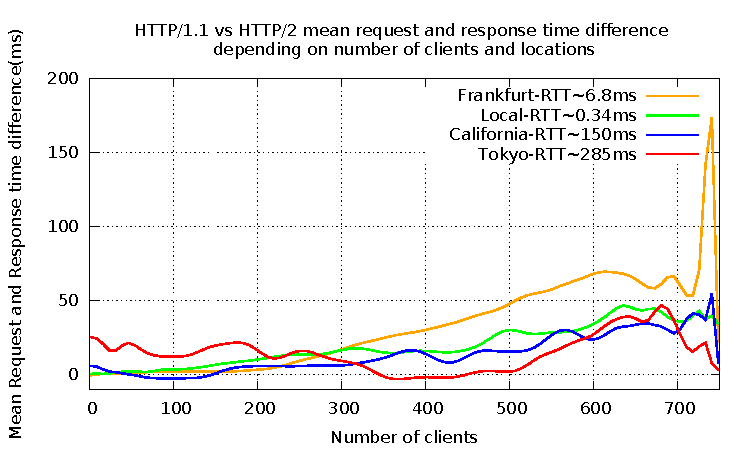
\includegraphics[scale=1,trim=0.0cm .0cm .0cm .0cm,clip]{images/difflatency.pdf}
	\caption{Mean RTT differences HTTP/1.1 - HTTP/2}
	\label{fig:latency-all}
\end{figure}


\subsection{Server Utilization}
\label{subsec:server_util}

During all measurements, CPU and network utilization on the server were monitored and measured. The different results can be categorized into low latency and high latency measurements. For that reason only the server utilization for the local (low latency) and North America (high latency) measurements will be presented. The performance graph for the server CPU utilization is shown in Figure \ref{fig:cpu}.  

\begin{figure}[H]
\centering
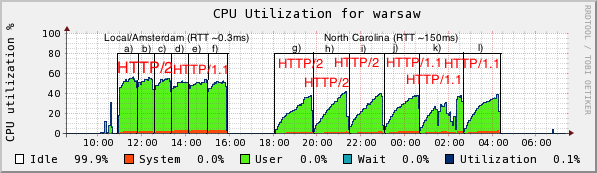
\includegraphics[scale=0.6,trim=0.0cm .0cm .0cm .0cm,clip]{images/cpu3.png}
\caption{Server CPU utilization for Local and North America measurements}
\label{fig:cpu}
\end{figure}

Table \ref{table:cpu} describes the corresponding annotations that have been made to point out which measurement belongs to which measurement parameters. That table applies also for the next performance graphs since we always show exactly the same time range in all following graphs.

\begin{table}[h]
	\centering
\begin{tabular}{ | c | c | c | }

\hline
\textbf{Index} &\textbf{Protocol} &\textbf{Web Page Size}\\ \hline \hline
a & HTTP/2 & small.html (20kB)\\ \hline
b & HTTP/2 & medium.html (600kB)\\ \hline
c & HTTP/2 & large.html (1600kB)\\ \hline
d & HTTP/1.1 & small.html (20kB) \\ \hline
e & HTTP/1.1 & medium.html (600kB) \\ \hline
f & HTTP/1.1 & large.html (1600kB)\\ \hline 
g & HTTP/2 & small.html (20kB)\\ \hline
h & HTTP/2 & medium.html (600kB)\\ \hline
i & HTTP/2 & large.html (1600kB)\\ \hline
j & HTTP/1.1 & small.html (20kB) \\ \hline
k & HTTP/1.1 & medium.html (600kB) \\ \hline
l & HTTP/1.1 & large.html (1600kB)\\  
\hline
\end{tabular}
\caption{Different Measurement parameters}
\label{table:cpu}
\end{table} 
 
The careful reader will now  notice that a medium.html web page shows up in Table \ref{table:cpu}. Indeed we created three different types of web pages. During the analysis of the data we realised that there is almost no significant difference in all measurements between the small size page and the medium size pages. For that reason we did not consider the measurements for the medium.html page and only focussed on the other two categories (large.html/small.html). However, in the performance graphs of the server the measurement for the medium size web pages are included.
\\ 
The left part of the graph shows the CPU utilization for local measurements (low latency) on the server and is annotated with the letters \textit{a} to \textit{f}. A sudden increase up to 60\% from the beginning on is remarkable until CPU utilization remains at a stable level. That correlates to the request rates graph for local measurements and nicely presents a high CPU utilization caused by the high number of requests towards the server. The measurements from \textit{a} to \textit{c} show HTTP/2 measurements and from \textit{d} to \textit{f} HTTP/1.1 measurements. A significant difference regarding CPU utilization is not noticeable. Starting from 6pm until 4am (annotated by \textit{g} to \textit{l}) measurements over a high latency link (North America) were performed. We see a constant growing of the CPU graph until the maximum number of clients of 750 for each test is reached. A nearly identical characteristic shows the bandwidth utilization graph. That correlates to the request per second graph as well and reflects a growing load caused by constantly increasing number of requests. A significant difference between HTTP/1.1 and HTTP/2 is also not noticeable for the high latency measurements. Furthermore a different load characteristic for changing sizes of web pages is not measurable for both protocol variants. 
\\
The traffic graph (Figure \ref{fig:network}) that represents the bandwidth utilization of the external interface of the server shows a similar characteristic compared to the CPU utilization graph (Figure \ref{fig:cpu}). One difference is the increased amount of traffic that can be explained by the increased amount of data for larger web pages. 

\begin{figure}[H]
\centering
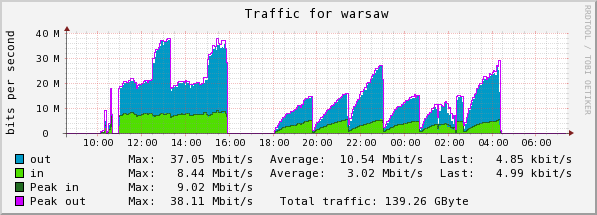
\includegraphics[scale=0.6,trim=0.0cm .0cm .0cm .0cm,clip]{images/network.png}
\caption{Server Bandwidth utilization for Local and North America measurements}
\label{fig:network}
\end{figure}

It is worth to mention that for all HTTP/1.1 measurements a lot of TCP TIME WAIT connections were discovered on the server. TCP TIME WAITS occur when the endpoint (server) blocks a current connection before it can close it due to some missing packets for that particular session. That happens because the server has many more TCP connections to manage for HTTP/1.1 compared to HTTP/2 and shows clearly the benefit of using the HTTP/2 protocol. 
The graph representing the TCP socket states on the server is shown in Figure \ref{fig:sockets}.

\begin{figure}[H]
\centering
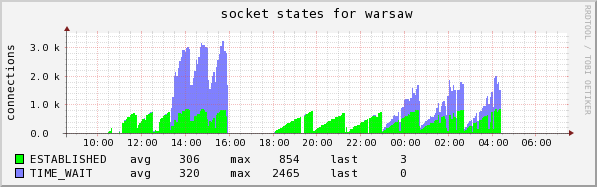
\includegraphics[scale=0.6,trim=0.0cm .0cm .0cm .0cm,clip]{images/sockets.png}
\caption{Server sockets for Local and North America measurements}
\label{fig:sockets}
\end{figure}
\newpage
\section{Conclusions}
\label{conclusion}

The research has identified differences between the HTTP/1.1 and HTTP/2 in terms of response and request time, amount of header data produced, possible request rates and impacts on the server utilization. A full benchmark setup has been developed consisting of several HTTP clients in different geographically locations and a server instance that delivers responses for both HTTP protocol versions. Moreover web pages of different sizes have been created to simulate "real-world" scenarios. In order to have accurate measurement results a benchmarking script \ref{sec:appendices} that makes use of h2load \cite{h2load} was deployed. 
\\
The measurements reflect the performance improvements a client will experience in the near future by using the new HTTP/2 protocol. Those improvements are mainly based on header compression mechanisms and more effective usage of TCP connections. Particularly high latency connections will benefit from the multiplexing mechanism that was introduced in HTTP/2. HTTP/2 will result in significant less TCP connection establishments (TCP three-way handshakes) on server side and thus it will save a lot of costly packet round trip times that would be required to fetch the same web page by using HTTP/1.1.
\\
A significant difference between HTTP/1.1 and HTTP/2 in terms of network load or CPU utilization was not detectable on the server. The main difference that has been discovered on server side is the TCP connection handling. It is faster and more effective when HTTP/2 is used, especially significantly less TCP TIME WAITS sockets were discovered on the server while performing HTTP/2 measurements.
\\
Large web service providers need to consider some technical implementation details when switching to the new protocol. First, so called deep inspection packet filters need to be adjusted in order to let HTTP/2 packets pass through. Those devices can no longer inspect HTTP/2 traffic on application level, as used to be the case with encrypted or unencrypted plain text HTTP/1.1 connections. The protocol is now binary and a simple telnet connection to a web server in order to conduct an HTTP GET request manually will not be possible with HTTP/2 anymore. Furthermore "hacks", like Sharding or Sprinting which were introduced in HTTP/1.1 to solve performance issues of the protocol are no longer necessary. In fact those HTTP/1.1 workarounds will lead to performance loss rather than to performance gain, if combined with HTTP/2.    


\newpage
\section{Further Work}
\label{furtherwork}

As it is a recent specification new implementations of the protocol will show up. Moreover the big players of server implementations such as NGINX\cite{nginx}} and apache \cite{apache2} have not implemented the protocol yet. But this is just a question of the time and probably they will wait until the protocol is specified in an RFC. In the meantime new implementations could be tested in comparison to see which one perform the best. At the time of writing the interesting server implementation of the protocol that are available are nghttp, H20, node-http2, openLiteSpeed. The list of all the implementations are available on the HTTP/2 github page.\cite{http2-imp}
Further work could be done by testing every new features of the protocol in order to show where are the improvement/drawbacks of this protocol in details per feature. 
HTTP/2 is still able to support HTTP/1.1 request with a proxy for legacy purposes. An interesting research subject could be how the  HTTP/1.1 legacy in HTTP/2 can slow down the adoption of the new version of protocol. This has been the case for IPv6 and by showing the improvements in performance for HTTP/2 it would be a pity to see legacy hold improvements in technology back again.
\newpage
\section*{}
\addcontentsline{toc}{section}{References}
\label{chap:references}
\begin{thebibliography}{99}
\bibitem{RFC723x}
RFC7230 Fielding, R., Ed., and J. Reschke, Ed., "Hypertext Transfer Protocol (HTTP/1.1): Message Syntax and Routing", RFC 7230, June 2014, Available at:http://www.rfc-editor.org/info/rfc7230  [Accessed 26 Mar. 2015]. \\
RFC7231 Fielding, R., Ed., and J. Reschke, Ed., "Hypertext Transfer Protocol (HTTP/1.1): Semantics and Content", RFC 7231, June 2014, Available at: http://www.rfc-editor.org/info/rfc7231 [Accessed 26 Mar. 2015]. \\
RFC7232 Fielding, R., Ed., and J. Reschke, Ed., "Hypertext Transfer Protocol (HTTP/1.1): Conditional Requests", RFC 7232, June 2014, Available at: http://www.rfc-editor.org/info/rfc7232 [Accessed 26 Mar. 2015]. \\ 
RFC7233 Fielding, R., Ed., Lafon, Y., Ed., and J. Reschke, Ed., "Hypertext Transfer Protocol (HTTP/1.1): Range Requests", RFC 7233, June 2014, Available at: http://www.rfc-editor.org/info/rfc7233 [Accessed 26 Mar. 2015]. \\
RFC7234 Fielding, R., Ed., Nottingham, M., Ed., and J. Reschke, Ed., "Hypertext Transfer Protocol (HTTP/1.1): Caching", RFC 7234, June 2014, Available at: http://www.rfc-editor.org/info/rfc7234 [Accessed 26 Mar. 2015]. \\
RFC7235 Fielding, R., Ed., and J. Reschke, Ed., "Hypertext Transfer Protocol (HTTP/1.1): Authentication", RFC 7235, June 2014, Available at: http://www.rfc-editor.org/info/rfc7235 [Accessed 26 Mar. 2015].
\bibitem{http2}
Hypertext Transfer Protocol version 2 (draft-ietf-httpbis-http2-17) (2015). M. Belshe, Twist R. Peon [online] IETF, Available at:
https://datatracker.ietf.org/doc/draft-ietf-httpbis-http2/?include\_text=1 [Accessed 26 Mar. 2015].
 \bibitem{hpack}
HPACK - Header Compression for HTTP/2 draft-ietf-httpbis-header-compression-07 (2015). R. Peon,  H. Ruellan [online] IETF, Available at: http://tools.ietf.org/html/draft-ietf-httpbis-header-compression-07 [Accessed 26 Mar. 2015].
\bibitem{stenberg}
Stenberg, D. (2015). http2 explained - The HTTP/2 book. [online] Daniel.haxx.se. Available at: http://daniel.haxx.se/http2/ [Accessed 27 Mar. 2015].
\bibitem{httpbis}
Tools.ietf.org, (2015). Httpbis Status Pages. [online] Available at: https://tools.ietf.org/wg/httpbis/ [Accessed 27 Mar. 2015].
\bibitem{spdy}
Google Developers, (2015). SPDY. [online] Available at: https://developers.google.com/speed/spdy/ [Accessed 27 Mar. 2015].
\bibitem{raymond}
Raymond, E. (2015). The Importance of Being Textual. [online] Catb.org. Available at: http://www.catb.org/esr/writings/taoup/html/ch05s01.html [Accessed 27 Mar. 2015].
\bibitem{curlhttp2}
Curl.haxx.se, (2015). cURL - README.http2. [online] Available at: http://curl.haxx.se/dev/readme-http2.html [Accessed 27 Mar. 2015].
\bibitem{wiresharkhttp2}
Wiki.wireshark.org, (2015). HTTP2 - The Wireshark Wiki. [online] Available at: https://wiki.wireshark.org/HTTP2 [Accessed 27 Mar. 2015].
\bibitem{breach}
Breachattack.com, (2015). BREACH ATTACK. [online] Available at: http://breachattack.com/ [Accessed 27 Mar. 2015].
\bibitem{crime}
Blackhat, (2013). A Perfect CRIME?. [online] Available at: https://media.blackhat.com/eu-13/briefings/Beery/bh-eu-13-a-perfect-crime-beery-wp.pdf [Accessed 27 Mar. 2015].
\bibitem{google2x}
A 2x Faster Web. (2009). [online] Chromium Blog. Available at: http://blog.chromium.org/2009/11/2x-faster-web.html [Accessed 20 Feb. 2015].
\bibitem{servy}
Servy, H. (2015). Evaluating the Performance of SPDY-enabled Web Servers. [online] Neotys.com. Available at: http://www.neotys.com/blog/performance-of-spdy-enabled-web-servers/ [Accessed 20 Feb. 2015].
\bibitem{podiatry}
Podiatry, G. (2015). Guy's Pod » Blog Archive » Not as SPDY as You Thought. [online] Guypo.com. Available at: http://www.guypo.com/not-as-spdy-as-you-thought/ [Accessed 20 Feb. 2015].
\bibitem{wang}
Wang et al. (2014). How Speedy is SPDY?, 11th USENIX Symposium on Networked Systems Design and Implementation (NSDI ’14). [online] usenix.org. Available at:
https://www.usenix.org/system/files/conference/nsdi14/nsdi14-paper-wang\_xiao\_sophia.pdf [Accessed 20 Feb. 2015].
\bibitem{amazon} Amazon Elastic Compute Cloud (Amazon EC2) (2015). Available at: http://aws.amazon.com/ec2/ [Accessed 20 Feb. 2015].
\bibitem{http2-imp}  HTTP/2 client/server implemenations (2015). Available at: https://github.com/http2/http2-spec/wiki/Implementations [Accessed 20 Feb. 2015].
\bibitem{h2c-14} Hypertext Transfer Protocol version 2 draft-ietf-httpbis-http2-14 (2014). Available at: https://tools.ietf.org/html/draft-ietf-httpbis-http2-14 [Accessed 4. March 2015]
\bibitem{nghttp} HTTP/2 experimental server (2015). Available at: https://nghttp2.org/documentation/nghttpd.1.html [Accessed 4. March 2015]
\bibitem{apache2} The Apache HTTP Server Project (2015). Available at: http://httpd.apache.org/ [Accessed 4. March 2015]
\bibitem{h2load} Benchmarking tool for HTTP/2 and SPDY server (2015). Available at: https://nghttp2.org/documentation/h2load.1.html [Accessed 4. March 2015]
\bibitem{httparchive} Httparchive.org, (2015). HTTP Archive - Trends. [online] Available at: http://httparchive.org/trends.php [Accessed 11 Mar. 2015].
\bibitem{nginx}
Garrett, O. (2015). How NGINX Plans to Support HTTP/2 - NGINX. [online] NGINX. Available at: http://nginx.com/blog/how-nginx-plans-to-support-http2/ [Accessed 27 Mar. 2015].
\bibitem{amazon-ts} amazon.com, (2015). Amazon - T2 Instances. [online] Available at: http://docs.aws.amazon.com/AWSEC2/latest/UserGuide/t2-instances.html [Accessed 11 Mar. 2015].
\bibitem{nghttpx} nghttp2.org, nghttpx a HTTP/1.1 HTTP/2 reverse proxy. [online] Available at: https://nghttp2.org/documentation/nghttpx.1.html [Accessed 1 April 2015].
\end{thebibliography}
\newpage
\section*{Appendices}
\addcontentsline{toc}{section}{Appendices}
\label{appendices}

\lstset{ % General setup for the package
	language=Perl,
	basicstyle=\small\sffamily,
	numbers=left,
 	numberstyle=\tiny,
	frame=tb,
	tabsize=4,
	columns=fixed,
	showstringspaces=false,
	showtabs=false,
	keepspaces,
	commentstyle=\color{gray},
	keywordstyle=\color{blue}
}

\begin{lstlisting}
#!/usr/bin/perl 
# Author Martin Leucht 2015 <martin.leucht@os3.nl>
#
# Benchmarking tool for HTTP/2 servers/reverse proxies
# based on h2load 
# https://nghttp2.org/documentation/h2load.1.html
#
# Usage: ./measure.pl [URL-list-file]
# Output is written to an CSV file

use List::Util qw(sum);
use strict;
use warnings;

my $file_urls = $ARGV[0];
my $runs=10;
my $stepsize_clients=2;
my $parallel_clients = 750;
my $bin_v2 = '/usr/local/bin/h2load';
my $start_datestring = gmtime();
my $time = time;
my $filename = "report_http_${file_urls}_${time}.csv";

sub check{
	my %units = ('1000' => 's','0.001' => 'us','1' => 'ms',);
	my $value = shift;
	my $unit = shift;
	
	foreach my $key (keys %units) {
		if ($units{$key} eq $unit) {
			our $ret = $key * $value;
			}
		}		
return our $ret;
}

sub average {
	my $size = @_;
	
	if ($size == 0) {
		print "NA";
		}
	else {return sum(@_)/@_;}
}


open(my $fh, '>', $filename) or die "Could not open file '$filename' $!";
print $fh "$start_datestring\n";
print $fh "number_of_requests,total_time_test,req_per_sec_v2,speed,traffic_total,traffic_header,
		   traffic_data,min_request,max_request,mean_request,sd_request,sd_percent_request,
		   succeeded_requests,succeeded_failed\n";
close $fh;



for (my $n=1; $n <= $parallel_clients; $n=$n+$stepsize_clients) {  
	my @finished_total_time_v2= ();
    my @finished_req_per_sec_v2 = ();
    my @finished_speed_v2 = ();
    my @finished_traffic_total_v2= ();
    my @finished_traffic_header_v2 = ();
    my @finished_traffic_data_v2 =();
    my @finished_min_request_v2 =();
    my @finished_max_request_v2 =();
    my @finished_mean_request_v2 =();
    my @finished_sd_request_v2 =();
    my @finished_sd_percent_request_v2 =();
    my @finished_succeeded =();
    my @finished_failed =();



	for (my $i=1; $i <= $runs; $i++) {
		
		my @command = `$bin_v2 -n $n -c $n --input-file=$file_urls --max-concurrent-streams=auto`;				
	
		foreach my $line (@command) {

			if ( $line =~ m/^finished.*?([0-9]*\.[0-9]*)(\w{1,2}).*?(\d+)\s.*?(\d+\.\d+).*/ ) {
				
				my $val = check($1,$2);	
				push(@finished_total_time_v2, $val);
				push(@finished_req_per_sec_v2, $3);
				push(@finished_speed_v2, $4);
				}
			elsif ( $line =~ m/^traffic.*?(\d+).*?(\d+).*?(\d+).*/ ) {	
				push(@finished_traffic_total_v2, $1);
                push(@finished_traffic_header_v2, $2);
                push(@finished_traffic_data_v2, $3);
				}
				
			elsif ( $line =~ m/^requests.*?(\d+)\s(?=succeeded).*?(\d+)\s(?=failed)/ ) {
				push(@finished_succeeded, $1);
				push(@finished_failed, $2);
				}	
					
			elsif ( $line =~ m/^time.*?(\d+\.*\d*)(\w{1,2}).*?(\d+\.*\d*)(\w{1,2}).*?(\d+\.*\d*)(\w{1,2}).*?(\d+\.*\d*)(\w{1,2}).*?(\d+\.*\d*).*/ ) {
				my $val1 = check($1,$2);
				my $val2 = check($3,$4);
				my $val3 = check($5,$6);
				my $val4 = check($7,$8);

                push(@finished_min_request_v2, $val1);
				push(@finished_max_request_v2, $val2);
				push(@finished_mean_request_v2, $val3);
				push(@finished_sd_request_v2, $val4);
				push(@finished_sd_percent_request_v2, $9);
				}
			else {print "";}
		}
	}	


	my $mean_finished_total_time_v2 = sprintf("%.4f", average(@finished_total_time_v2));
	my $mean_finished_req_per_sec_v2 = sprintf("%.2f",average(@finished_req_per_sec_v2));
	my $mean_finished_speed_v2 = sprintf("%.2f",average(@finished_speed_v2));
	my $mean_finished_traffic_total_v2 = sprintf("%.0f",average(@finished_traffic_total_v2));
	my $mean_finished_traffic_header_v2 = sprintf("%.0f",average(@finished_traffic_header_v2));
	my $mean_finished_traffic_data_v2 = sprintf("%.0f",average(@finished_traffic_data_v2));
	my $mean_finished_min_request_v2 = sprintf("%.4f",average(@finished_min_request_v2));
	my $mean_finished_max_request_v2 = sprintf("%.4f",average(@finished_max_request_v2));
	my $mean_finished_mean_request_v2 = sprintf("%.4f",average(@finished_mean_request_v2));
	my $mean_finished_sd_request_v2 = sprintf("%.4f",average(@finished_sd_request_v2));
	my $mean_finished_sd_percent_request_v2 = sprintf("%.2f",average(@finished_sd_percent_request_v2));
	my $mean_finished_succeeded_v2 = sprintf("%.0f",average(@finished_succeeded));
	my $mean_finished_failed_v2 = sprintf("%.0f",average(@finished_failed));
	
	open(my $fh, '>>', $filename) or die "Could not open file '$filename' $!";
    print $fh "$n,$mean_finished_total_time_v2,$mean_finished_req_per_sec_v2,
    			$mean_finished_speed_v2,$mean_finished_traffic_total_v2,$mean_finished_traffic_header_v2,
    			$mean_finished_traffic_data_v2,$mean_finished_min_request_v2,$mean_finished_max_request_v2,
    			$mean_finished_mean_request_v2,$mean_finished_sd_request_v2,$mean_finished_sd_percent_request_v2,
    			$mean_finished_succeeded_v2,$mean_finished_failed_v2\n";
    close $fh;
		
}			

my $end_datestring = gmtime();
open(my $fh, '>>', $filename) or die "Could not open file '$filename' $!";
print $fh "$end_datestring\n";
close $fh;

			
\end{lstlisting}


\end{document}
